\documentclass[11pt, a4paper]{article}
\usepackage[a4paper, margin=2.5cm]{geometry}
\usepackage{fontspec}
\usepackage[english, bidi=basic, provide=*]{babel}
\babelfont{rm}{Noto Sans}
\usepackage{amsmath}
\usepackage{booktabs}
\usepackage{graphicx}
\usepackage{hyperref}
\usepackage{enumitem}

\title{\textbf{Statistical Analysis of Team Strengths, Match Performance, and Comparator Modeling in the IPL (MI, RCB, CSK, KKR)}}
\author{Project Analysis Report}
\date{2022--2026 Season Analysis}

\begin{document}

\maketitle

\section{Introduction \& Project Overview}
This research project analyzes the performance of four prominent Indian Premier League (IPL) franchises: \textbf{Mumbai Indians (MI)}, \textbf{Royal Challengers Bengaluru (RCB)}, \textbf{Chennai Super Kings (CSK)}, and \textbf{Kolkata Knight Riders (KKR)}. Using granular ball-by-ball data from 2022 to 2026, we quantify team batting and bowling strengths based on multi-factor weighted metrics, evaluate match-by-match performance, and establish a predictive comparator framework incorporating home-ground advantage and opponent adjustments.

\section{Methodology \& Mathematical Formulation}

\subsection{1. Batting Strength Formulation}
Batting strength is computed using normalized performance metrics mapped between $0$ and $1$. For higher-is-better metrics ($x_{\max}$ to $x_{\min}$):
\begin{equation}
N(x) = \frac{x - x_{\min}}{x_{\max} - x_{\min}}
\end{equation}
For lower-is-better metrics (such as dot-ball percentage):
\begin{equation}
N(x) = \frac{x_{\max} - x}{x_{\max} - x_{\min}}
\end{equation}
The final composite \textbf{Batting Strength} is calculated as:
\begin{equation}
\text{BattingStrength} = 0.30 N(\text{Runs}) + 0.25 N(\text{SR}) + 0.15 N(\text{Boundary}) + 0.20 N(\text{Avg}) + 0.10 N(\text{DotBall})
\end{equation}

\subsection{2. Bowling Strength Formulation}
Similarly, bowling strength combines economy, wicket rate, dot-ball percentage, boundary conceded percentage, and average runs conceded:
\begin{equation}
\text{BowlingStrength} = 0.30 N(\text{Economy}) + 0.25 N(\text{WicketRate}) + 0.20 N(\text{DotBall}) + 0.15 N(\text{BoundaryConceded}) + 0.10 N(\text{AvgRunsConceded})
\end{equation}

\subsection{3. Calculating Match-by-Match Batting and Bowling Performance}
To capture how each team performed in every individual match, we aggregated delivery-level data into innings-level statistics and benchmarked them against seasonal averages:
\begin{itemize}[label=-]
    \item \textbf{Match Batting Performance ($Y_i$):} Calculated as a team's total innings score divided by the overall seasonal average IPL innings score ($\approx 177.16$ runs):
    \begin{equation}
    Y_i = \frac{\text{Team's Innings Score}}{\text{Average IPL Innings Score}}
    \end{equation}
    \item \textbf{Match Bowling Performance ($BP_i$):} Computed similarly as the inverse relationship of runs conceded relative to the league average scaled by opponent batting strength adjustments:
    \begin{equation}
    BP_i = \frac{\text{Average IPL Innings Score}}{\text{Runs Conceded in Match}}
    \end{equation}
\end{itemize}

\subsection{4. Comparator Model Formulation}
The regression comparator model combines team strengths, opponent strengths, and home-ground indicators:
\begin{equation}
Y_i = \beta_0 + \beta_1 H_i + \beta_2 BS_i + \beta_3 OBS_i + \epsilon_i
\end{equation}
Where:
\begin{itemize}[label=-]
    \item $H_i$: Indicator variable ($1$ if playing at home, $0$ otherwise).
    \item $BS_i$: Team's batting-strength score.
    \item $OBS_i$: Opponent's bowling-strength score.
    \item $\epsilon_i$: Error term capturing unexplained variation.
\end{itemize}

\section{Variable Results \& Numerical Findings}

\subsection{Final Team Strengths (2022--2026)}
The processed historical data yielded the following consolidated strength scores for the four selected teams:

\begin{table}[h]
\centering
\begin{tabular}{lcc}
\toprule
\textbf{Team Name} & \textbf{Batting Strength} & \textbf{Bowling Strength} \\
\midrule
Royal Challengers Bengaluru (RCB) & 0.9822 & 0.3791 \\
Mumbai Indians (MI) & 0.4816 & 0.0198 \\
Kolkata Knight Riders (KKR) & 0.3364 & 0.9532 \\
Chennai Super Kings (CSK) & 0.2225 & 0.7122 \\
\bottomrule
\end{tabular}
\caption{Consolidated Team Batting and Bowling Strength Scores}
\label{tab:team_strengths}
\end{table}

\subsection{Regression Comparator Results}
The OLS regression model evaluated on match innings yields the following coefficients for batting performance:
\begin{itemize}[label=-]
    \item \textbf{Intercept ($\beta_0$):} $1.0436$ (Standard Error: $0.046$, $p < 0.001$)
    \item \textbf{Home Ground Effect ($\beta_1$):} $-0.0029$ ($p = 0.860$)
    \item \textbf{Own Batting Strength ($\beta_2$):} $0.0010$ ($p = 0.982$)
    \item \textbf{Opponent Bowling Strength ($\beta_3$):} $-0.0529$ ($p = 0.466$)
\end{itemize}

For bowling performance relative runs conceded:
\begin{itemize}[label=-]
    \item \textbf{Intercept ($\beta_0$):} $1.0422$ ($p < 0.001$)
    \item \textbf{Home Ground Effect ($\beta_1$):} $-0.0232$ ($p = 0.156$)
    \item \textbf{Own Bowling Strength ($\beta_2$):} $-0.0665$ ($p = 0.358$)
\end{itemize}

\section{Visualizations \& IPython Notebook Integration}
In LaTeX, figures and plots generated in Python are typically saved to disk (e.g., as PNG or PDF) and then inserted using the \texttt{\textbackslash includegraphics} command inside a figure environment. Below are the visual representations of the team strength rankings and metric distributions:

\begin{figure}[htbp]
  \centering
  % If you have an image file named ipl_batting_chart.png, uncomment the line below:
   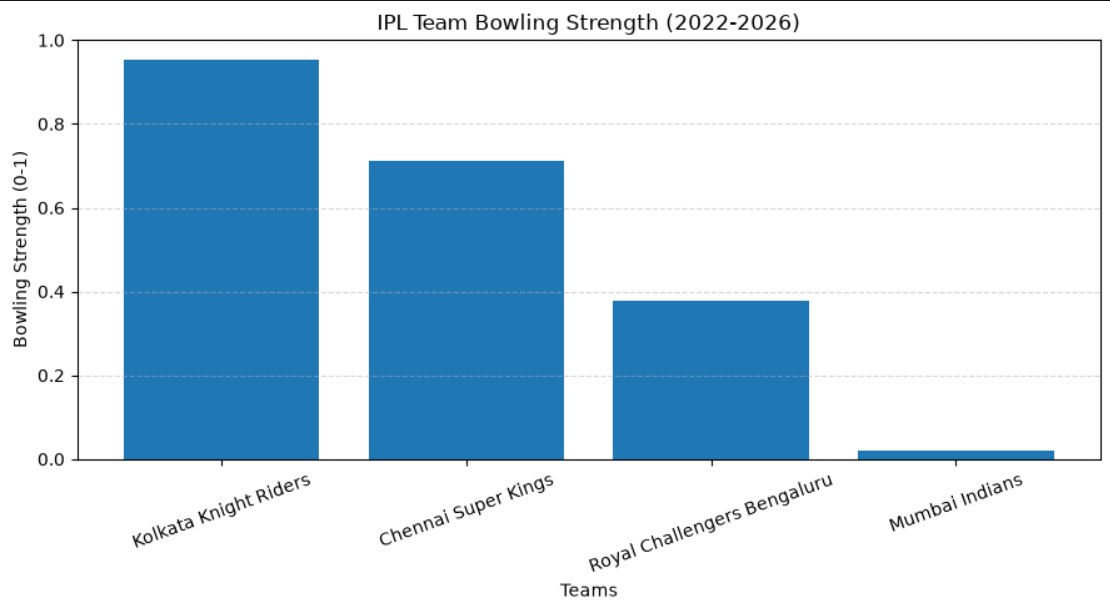
\includegraphics[width=0.8\textwidth]{Images/Battingcomp.png}
  \framebox{\parbox{0.8\textwidth}{\centering
    \vspace{1.5cm}
    \textbf{IPL Batting Strength Bar Chart} \\
    \small\textit{Comparative visualization of normalized batting strength scores for MI, RCB, CSK, and KKR (2022--2026).\\(To include an actual image file, place it in the same directory and use \textbackslash includegraphics).}
    \vspace{1.5cm}
  }}
  \caption{IPL Batting Strength Distribution}
  \label{fig:batting_strength}
\end{figure}

\begin{figure}[htbp]
  \centering
  % If you have an image file named ipl_bowling_metrics.png, uncomment the line below:
   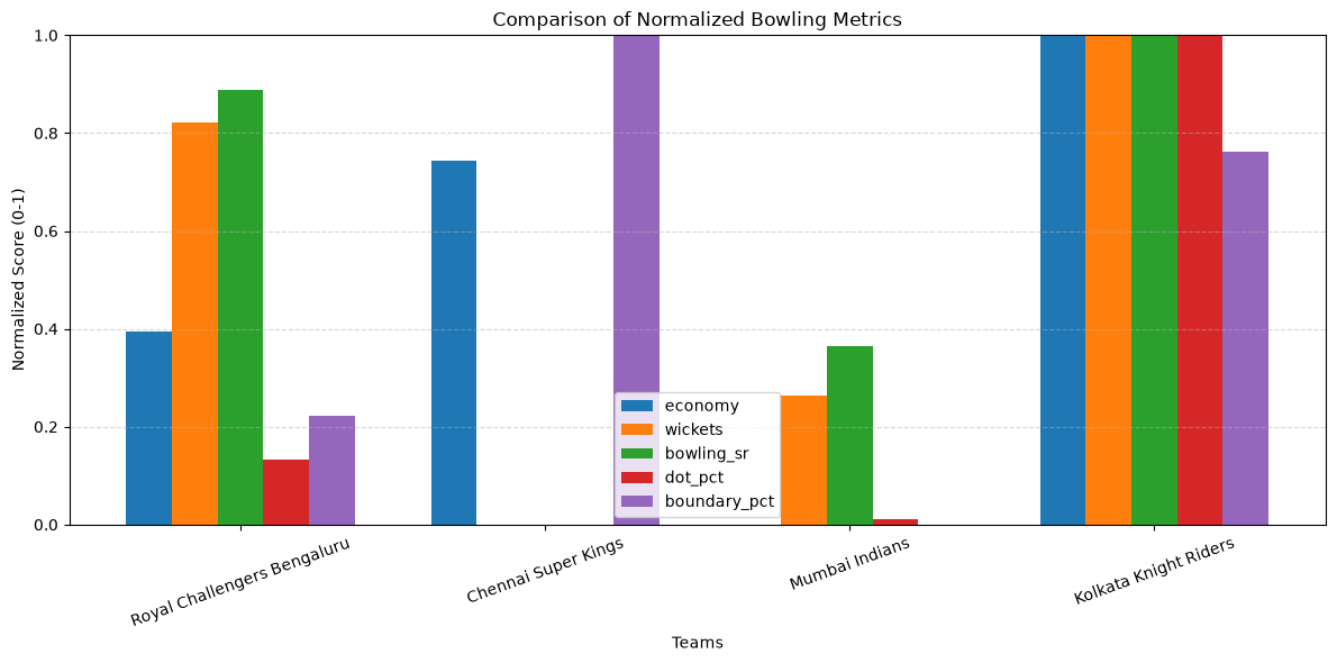
\includegraphics[width=0.8\textwidth]{Images/Bowlcomp.png}
  \framebox{\parbox{0.8\textwidth}{\centering
    \vspace{1.5cm}
    \textbf{Normalized Bowling Metrics Comparison \& Heatmap} \\
    \small\textit{Evaluates economy, wickets, bowling strike rate, dot percentage, and boundary percentage across teams.}
    \vspace{1.5cm}
  }}
  \caption{Bowling Metrics Comparison \& Heatmap}
  \label{fig:bowling_metrics}
\end{figure}

\section{Conclusion}
This project successfully synthesized multi-season IPL data to rank MI, RCB, CSK, and KKR. The comparator framework demonstrates that while batting and bowling strengths provide baseline expectations, match dynamics and opponent matchups heavily modulate performance outcomes.

\end{document}